Avant de commencer voici la strucure globale de notre projet :
\begin{itemize}
   \item le fichier \lstinline{pagerank.adb} est notre code principal
   \item le module \lstinline{helpers} contient toutes les fonctions tierses ne faisant pas partie intégrante de Google, pouvant s'externaliser afin de décharger le fichier \lstinline{pagerank.adb}.
   \item de même le module \lstinline{exceptions} définit toutes les exceptions du projet
   \item les modules \lstinline{google}, \lstinline{google_naive} et \lstinline{google_creuse} implémentant les différantes versions du code.
\end{itemize}

L'avantage d'externaliser les modules \lstinline{exceptions} et \lstinline{helpers} est que l'on peut se servir de leur contenu à la fois dans le module \lstinline{google} et dans le fichier \lstinline{pagerank.adb}.

\begin{figure}[ht!]
   \centering
   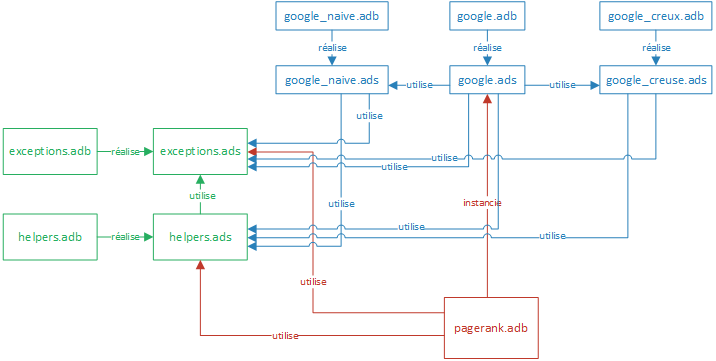
\includegraphics[scale=0.8]{partie-2/sous-partie-1/architecture.png}
   \caption{Architecture du projet \label{fig : architecture_projet}}
\end{figure}